\documentclass[letterpaper,11pt]{article}

\usepackage{latexsym}
\usepackage[empty]{fullpage}
\usepackage{titlesec}
\usepackage{marvosym}
\usepackage[usenames,dvipsnames]{color}
\usepackage{verbatim}
\usepackage{enumitem}
\usepackage[hidelinks]{hyperref}
\usepackage{fancyhdr}
\usepackage[english]{babel}
\usepackage{tabularx}
\usepackage{fontawesome5}
\usepackage{multicol}
\setlength{\multicolsep}{-3.0pt}
\setlength{\columnsep}{-1pt}
\input{glyphtounicode}

%new packages

\usepackage{fontenc}
\usepackage{amsmath}
\usepackage{amssymb}
\usepackage{graphicx}



%----------FONT OPTIONS----------

\pagestyle{fancy}
\fancyhf{} % clear all header and footer fields
\fancyfoot{}
\renewcommand{\headrulewidth}{0pt}
\renewcommand{\footrulewidth}{0pt}

% Adjust margins
\addtolength{\oddsidemargin}{-0.6in}
\addtolength{\evensidemargin}{-0.5in}
\addtolength{\textwidth}{1.19in}
\addtolength{\topmargin}{-.7in}
\addtolength{\textheight}{1.4in}

\urlstyle{same}

\raggedbottom
\raggedright
\setlength{\tabcolsep}{0in}

% Sections formatting
\titleformat{\section}{
  \vspace{-4pt}\scshape\raggedright\large\bfseries
}{}{0em}{}[\color{black}\titlerule \vspace{-5pt}]



% Ensure that generate pdf is machine readable/ATS parsable
\pdfgentounicode=1

%-------------------------
% Custom commands
\newcommand{\resumeItem}[1]{
  \item\small{
    {#1 \vspace{-2pt}}
  }
}

\newcommand{\classesList}[4]{
    \item\small{
        {#1 #2 #3 #4 \vspace{-2pt}}
  }
}

\newcommand{\resumeSubheading}[4]{
  \vspace{-2pt}\item
    \begin{tabular*}{1.0\textwidth}[t]{l@{\extracolsep{\fill}}r}
      \textbf{#1} & \textbf{\small #2} \\
      \textit{\small#3} & \textit{\small #4} \\
    \end{tabular*}\vspace{-7pt}
}

\newcommand{\resumeSubSubheading}[2]{
    \item
    \begin{tabular*}{0.97\textwidth}{l@{\extracolsep{\fill}}r}
      \textit{\small#1} & \textit{\small #2} \\
    \end{tabular*}\vspace{-7pt}
}

\newcommand{\resumeProjectHeading}[2]{
    \item
    \begin{tabular*}{1.001\textwidth}{l@{\extracolsep{\fill}}r}
      \small#1 & \textbf{\small #2}\\
    \end{tabular*}\vspace{-7pt}
}


\newcommand{\resumeSubItem}[1]{\resumeItem{#1}\vspace{-4pt}}

\renewcommand\labelitemi{$\vcenter{\hbox{\tiny$\bullet$}}$}
\renewcommand\labelitemii{$\vcenter{\hbox{\tiny$\bullet$}}$}

\newcommand{\resumeSubHeadingListStart}{\begin{itemize}[leftmargin=0.0in, label={}]}
\newcommand{\resumeSubHeadingListEnd}{\end{itemize}}
\newcommand{\resumeItemListStart}{\begin{itemize}}
\newcommand{\resumeItemListEnd}{\end{itemize}\vspace{-5pt}}



\begin{document}
\fontfamily{cmr}\selectfont
\begin{center}
\parbox{3.0cm}{%
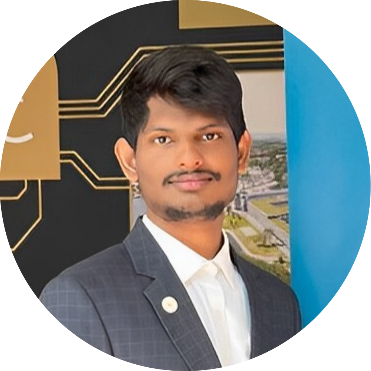
\includegraphics[width=2.7cm,clip]{images/resume_pic_m.png}}
}
\parbox{\dimexpr\linewidth-3.8cm\relax}{
\vspace{-20pt}
\begin{tabularx}{\linewidth}{L r} \\
    {\Huge \scshape Venkata Sai Yakkshit Reddy Asodi}~
    \href{https://www.cedzlabs.com/yakkshit}{\vspace{1pt}}\\
      Berlin, Germany. \\ \vspace{1pt}
     \small \raisebox{-0.1\height}\faPhone\ +91 8179936156 ~ \href{mailto:saiyakkshit2001@gmail.com}{\raisebox{-0.2\height}\faEnvelope\ {saiyakkshit2001@gmail.com}} ~ 
    \href{https://linkedin.com/in/yakkshit/}{\raisebox{-0.2\height}\faLinkedin\ {yakkshit}}  ~
    \href{https://yakkshit.com/}{\raisebox{-0.2\height}\faGlobe\ {yakkshit.com}}  ~
    \href{https://github.com/yakkshit}{\raisebox{-0.2\height}\faGithub{ yakkshit}}
    \vspace{-8pt}
    
\end{tabularx}
}
\end{center}

\vspace{-23pt}

\section{Summary \faLink}
Dynamic Full Stack Developer with expertise in JavaScript, React, Node.js, and PostgreSQL. Proven track record of developing scalable applications and leading development teams. Passionate about building innovative solutions to digitize businesses and enhance consumer experiences.

\section{Technical Skills \faLink}
\begin{itemize}[leftmargin=0.15in, label={}]
\small{\item{
\textbf{Languages - }{JavaScript, TypeScript, HTML, CSS, Python.} \\
\textbf{Frameworks - }{React, Node.js, Express, Next.js.} \\
\textbf{Databases - }{PostgreSQL, MongoDB.} \\
\textbf{Cloud - }{AWS, Azure.} \\
\textbf{Tools - }{Docker, Git, Postman.} \\
\textbf{APIs - }{REST, GraphQL.} \\
}}
\end{itemize}
\vspace{-10pt}

\section{Experience \faLinkedin}
\resumeSubHeadingListStart

\resumeSubheading
{\large Circleup AG}{January 2024 -- Present}
  {Lead Full Stack Engineer}{Zurich, Switzerland}\\
\vspace{10pt}
\textbf{Responsibilities:}
\resumeItemListStart
\vspace{-10pt}
\resumeItem{Led front-end and back-end development, building scalable web applications using React and Django.}
\resumeItem{Collaborated with product teams to design and implement user-centered features.}
\resumeItem{Integrated APIs and cloud-based services, optimizing application performance and security.}
\resumeItemListEnd
\vspace{-3pt}
\textbf{Environment:}\emph{React, Django, AWS, PostgreSQL, Agile.}

\resumeSubheading
{Cedzlabs}{March 2023 -- December 2023}
{Full Stack Developer}{India (Remote)}\\
\vspace{10pt}
\textbf{Responsibilities:}
\resumeItemListStart
\vspace{-10pt}
\resumeItem{Developed intuitive, responsive front-end components for a SaaS platform using React and Next.js.}
\resumeItem{Integrated server-side logic and database management with Node.js and PostgreSQL.}
\resumeItem{Ensured cross-browser compatibility and responsive designs for web applications.}
\resumeItemListEnd
\vspace{-3pt}
\textbf{Environment:}\emph{React, Next.js, PostgreSQL, Docker, AWS.}

\resumeSubHeadingListEnd

\section{Projects \faGithub}
\resumeSubHeadingListStart
\resumeProjectHeading
{\textbf{\href{https://ui.cedzlabs.com}{Ondasera Digital Platform}} $|$ \emph{React, Node.js, PostgreSQL, AWS}}{January 2024 -- Present}\\
\vspace{6pt}
\textbf{Description:}
\vspace{-5pt}
\resumeItemListStart
\resumeItem{Led the development of a digital platform that connects cemeteries and their partners, automating workflows and enhancing consumer interactions.}
\resumeItem{Designed the architecture for scalable back-end services using Node.js and PostgreSQL.}
\resumeItem{Deployed cloud infrastructure on AWS for high availability and secure data storage.}
\resumeItemListEnd
\vspace{4pt}
\textbf{Tools:}\emph{React, Node.js, PostgreSQL, AWS.}

\resumeProjectHeading
{\textbf{\href{https://yakkshit.com}{AI Resume Tuner}} $|$ \emph{Next.js, Azure, LLMs}}{August 2023}\\
\vspace{6pt}
\textbf{Description:}
\vspace{-5pt}
\resumeItemListStart
\resumeItem{Built an AI-powered resume tuner that customizes resumes using job descriptions, leveraging LLMs for content optimization.}
\resumeItem{Deployed on Azure for scalability and secure handling of user data.}
\resumeItemListEnd
\vspace{4pt}
\textbf{Tools:}\emph{Next.js, Azure, LLMs.}

\resumeSubHeadingListEnd

\section{Achievements}
\resumeItemListStart
\resumeItem{Successfully led full stack development for SaaS platforms, resulting in optimized user experiences and increased revenue.}
\resumeItem{Contributed to open-source projects related to web development and cloud technologies.}
\resumeItem{Regularly participate in hackathons and won prizes for innovative solutions.}
\resumeItemListEnd

\section*{Languages}
\begin{itemize}
  \item English - Fluent $|$ Hindi - Fluent $|$ Telugu - Native $|$ German - Elementary
\end{itemize}

\vspace{10pt}
\end{document}